% !TEX root = DauceAlbigesPerrinet2020.tex
% !TEX encoding = UTF-8 Unicode
% -*- coding: UTF-8; -*-
% vim: set fenc=utf-8
% !TEX spellcheck = en-US
%=================================================================
\section{Methods}
\label{sec:implementation}
%To test the validity of our hypothesis, let us find a function implementing the ``Where'' network. This function should be able to find the position of an object knowing only the degraded retinal image. Here, we describe the methods that we will follow to find that function, from the generative models (first external and then internal) to the actual implementation of the ``Where'' pathway. %

\subsection{Image generation}
%=================================================================
We first define here the generative model for input display images as shown first in Figure~\ref{fig:intro}-A (\DIS ) and as implemented in Figure~\ref{fig:methods}-A. Following a common hypothesis regarding active vision, visual scenes consist of a single target embedded in a large image with a cluttered background.

\paragraph{Targets.}
We use the MNIST dataset of handwritten digits introduced by~\cite{Lecun1998}: %Indeed, we are here focused on the problem of localization (``Where'' pathway) and classification solutions (``What'' pathway) abound for this class of targets.
Samples are drawn from the dataset of $60000$ grayscale $28\times 28$ pixels images and separated between a training and a validation set (see below the description of the ``Where'' network).
% {\color{red} \textbf{Rev 2} The foveal processing module does a 10-way classification. But what about a no-digit example? Does the model predict “no-digit” or “background”? Is there a need for such a decision? Please discuss.}
% Note that to simplify the task there is one and only one target in the image.

\paragraph{Full-scale images.}
Input images are full-scale images of size $128\times 128$ in which we embed the target.
Each target location is drawn at random in this large image. To enforce isotropic generation (at any direction from the fixation point), a centered circular mask covering the image (of radius $64$ pixels) is defined, and the target's location is such that the embedded sample fits entirely into that circular mask.

\paragraph{Background noise setting.} To implement a realistic background noise, we generate synthetic textures~\cite{Sanz12} using a bi-dimensional random process. %The generated texture images are of the same size than the full-image.
The texture is designed to fit well with the statistics of natural images. We chose an isotropic setting where textures are characterized by solely two parameters, one controlling the median spatial frequency of the noise, the other controlling the bandwidth around the central frequency. Equivalently, this can be considered as the band-pass filtering of a random white noise image. The spatial frequency is set at $0.1\text{ pixel}^{-1}$ to fit that of the original digits. This specific spatial frequency occasionally allows to generate some ``phantom'' digit shapes in the background. Finally, these images are rectified to have a normalized contrast.

\paragraph{Mixing the signal and the noise.} Finally, both the noise and the target image are merged into a single image. Two different strategies are used. A first strategy emulates a transparent association, with an average luminance computed at each pixel, while a second strategy emulates an opaque association, choosing for each pixel the maximal value. The quantitative difference was tested in simulations, but proved to have a marginal importance.

\subsection{Active inference and the Naïve Bayes assumption}

%{\color{blue} {\bf rev 2} Throughout the text, the variable “x” is described in several different ways: (i) state of sensor, (ii)  partial view of the scene, (iii) visual field, and (iv) visual sample. This might be confusing to the reader. Please be consistent. {\bf laurent:} tu as pu regarder ce point?}

Saccade selection in visual processing can be captured by a statistical framework called a
partially observed Markov Decision Process (POMDP)~\cite{Najemnik05,Butko2010infomax,Friston12}, where the cause of a visual scene is  made up from the couple of independent random variables of the viewpoint and of the scene elements (here a digit). For instance, changing the viewpoint will conduct to a different scene rendering.
A generative model tells how the visual field should look knowing the scene elements and a certain viewpoint.
In general, active inference assumes a hidden external state $e$, which is known indirectly through its effects on the sensor. The external state corresponds to the physical environment. Here the external state is assumed to split in two (independent) components, namely $e = (u,y)$ with $u$ the interoceptive body posture (in our case the gaze orientation, or ``viewpoint'') and $y$ the object shape (or object identity). The visual field $x$ is the state of the sensors, that is, a partial view of the visual scene, measured through the generative process : $x\sim p(X|e)$.


Using Bayes rule, one may then infer the scene elements from the current viewpoint (model inversion).
 The real physical state $e$ being hidden, a parametric model $\theta$ is assumed to allow for an estimate of the cause of the current visual field through model inversion thanks to Bayes formula, in short:
$$p(E|x) \propto p(x|E;\theta)$$


It is also assumed that a set of motor commands $A = \{..., a, ...\}$ (here saccades) may control the body posture, but not the object's identity, so that $y$ is invariant to $a$. Actuating a command $a$ changes the viewpoint to $u'$, which feeds the system with a new visual sample $x'\sim p(X|u', y)$. The more viewpoints you have, the more certain you are about the object identity through a chain rule sequential evidence accumulation.

In an optimal search setup however~\cite{Najemnik05}, you need to choose the next viewpoint that will help you \emph{the most} to disambiguate the scene.
In a predictive setup, the consequence of every saccade should be analyzed through model inversion \emph{over the future observations}, that is, predicting the effect of every action to choose the one that may optimize future inferences. The benefit of each action should be quantified through a certain metric (future accuracy, future posterior entropy, future variational free energy, ...), that depend on the current inference $p(U,Y|x)$. The saccade $a$ that is selected thus provides a new visual sample from the scene statistics. If well chosen, it should improve the understanding of the scene (here the target position and category). However, estimating in advance the effect of every action over the range of every possible object shapes and body postures is combinatorially hard, even in simplified setups, and thus infeasible in practice.

%To infer the position of the target, we will use the fundamental hypothesis outlined in Figure~\ref{fig:intro}: The position of an object is independent from its category.
The predictive approach necessitates in practice to restrain the generative model in order to reduce the range of possible combinations. One such restriction, known as the ``Naïve Bayes'' assumption, considers the independence of the factors that are the cause of the sensory view.
The independence hypothesis allows considering the viewpoint $u$ and the category $y$ being independently inferred from the current visual field, i.e $p(U,Y|x) = p(U|x) p(Y|x)$. This property is strictly true in our setting and is very generic in vision for simple classes (such as digits) and simple displays (but see~\cite{Vo12} for more complex visual scene grammars).
%

%
\subsection{Foveal vision and the ``What'' pathway}
%=================================================================
%
At the core of the vision system is the identification module, i.e. the ``What'' pathway (see fig. \ref{fig:methods}). It consists of a classic convolutional classifier for which we will show some translation invariance in the form of a shift-dependent accuracy map. Importantly, it can quantify its own classification uncertainty, that may allow comparisons with the output of the ``Where'' pathway.

The foveal input is defined as the $28\times 28$ grayscale image cropped at the center of gaze (see dashed red box in Figure~\ref{fig:intro}-C).
This image is passed unmodified to the agent's visual categorical pathway (the ``What'' pathway), that is realized by a convolutional neural network, here the well-known ``LeNet'' classifier~\cite{Lecun1998}. The network structure that processes the input to identify the target category is made of 3 convolution layers interleaved with max-pooling layers, followed by two fully-connected layers as provided (and unmodified) by the Pytorch library~\cite{NEURIPS2019_9015}. Each intermediate layer's output is rectified and
% {\color{red} \textbf{rev 2} Authors claim the foveal processing has some translational invariance. However, they do not mention the use of any pooling layers in the convolutional net. Are there any pooling layers? If not, how does the conv net achieve translation invariance? Would not it be better to use max-pooling?  The architecture of the conv net is not given in the paper. And from the reference [26], I could not find it. Care must be taken when formatting the references. If the reference is a web-page, its URL must be given along with its last accessed date. }
the network output uses a sigmoid operator to represent the probability of detecting each of the $10$ digits. The index of one of the 10 output neuron with maximum probability provides the image category.
It is first trained over the (centered) MNIST dataset after approx $20$ training epochs. %Input images are rectified (\emph{with a mean and standard deviation of respectively $0.1307$ and $0.3081$ {\bf why??}}).} \fi
This strategy achieves an average $98.7\%$ accuracy on the validation dataset~\cite{Lecun1998}.%

\begin{figure}[t!]%%[p!]
	\centering{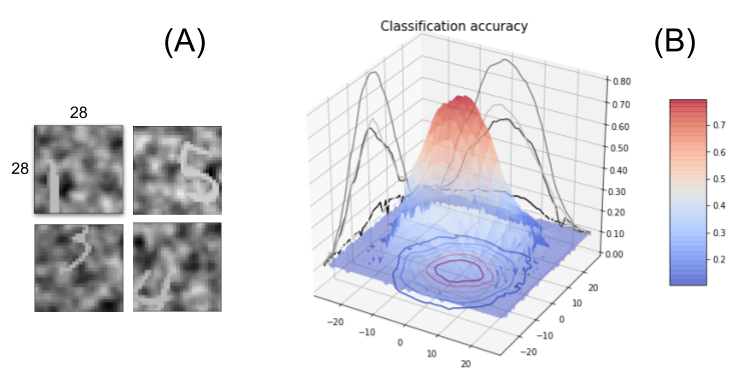
\includegraphics[width=\linewidth]{fig_what_accmap.png}}
	\caption{\A Input samples from the ``What'' training set, with  randomly shifted targets using a Gaussian bivariate spatial shift with a standard deviation of 15 pixels. The target contrast is randomly set between 30~\% and 70~\%.
	\B $55 \times 55$ shift-dependent accuracy map, measured for different target eccentricities on the test set after training.
	}
\label{fig:accuracy}
\end{figure}

% TODO repasser une couche sur cette partie que je maitrise moins
To achieve a more generic ``What'' pathway, a specific dataset is constructed to train the network. It is made of randomly shifted digits overlayed over a randomly generated noisy background, as defined above. Both the shift, the contrast and the background noise make the task more difficult than the original MNIST categorization. The relative contrast of the digit is randomly set between 30~\% and 70~\% of the maximal contrast.  The network is trained incrementally by progressively increasing the shift variability (of a bivariate central gaussian) and by increasing the standard deviation from $0$ to $15$ (with a maximal shift set at $27$ pixels). The network is trained on a total of $75$ epochs, with $60000$ examples generated at each epoch from the original MNIST training set. The shifts and backgrounds are re-generated at each epoch. The shifts' standard deviation increases of one unit every $5$ epochs such that at the end of the training, many digits fall outside the center of the fovea, so that many examples are close to impossible to categorize, either because of a low contrast or a too large eccentricity. At the end of the training process, the average accuracy is thus of $34\%$ and a maximum accuracy $91\%$ at the center.

After training, this shift-dependent accuracy map is validated by systematically testing the network accuracy on every horizontal and vertical shift, each on a set of $1000$ cluttered target samples generated from the MNIST test set and within the range of $\pm 27$ pixels (see figure~\ref{fig:accuracy}).  This forms a $55\times 55$ accuracy map showing higher accuracy at the center, and a slow decreasing accuracy with target eccentricity (with an accuracy plateau  over $70\%$ showing a relative shift invariance on around $7$ pixels eccentricity radius). This shift invariance is a known effect of convolutional computation. Note that the categorization task is here harder by construction and the accuracy that is obtained here is lower (with a central recognition rate of around $80\%$). The accuracy sharply drops for eccentricities  greater than $10$ pixels, reaching the baseline $10\%$ chance level at shift amplitudes at around $20$ pixels.
%, as shown in(with a central value of $80\%$ corresponding to the validation score without any translational shift),

\subsection{``Where'' pathway: Transforming log-polar feature vectors to log-polar action maps}

\begin{figure}[t!]%%[p!] (see Figure~\ref{fig:where}-C)
	\centering{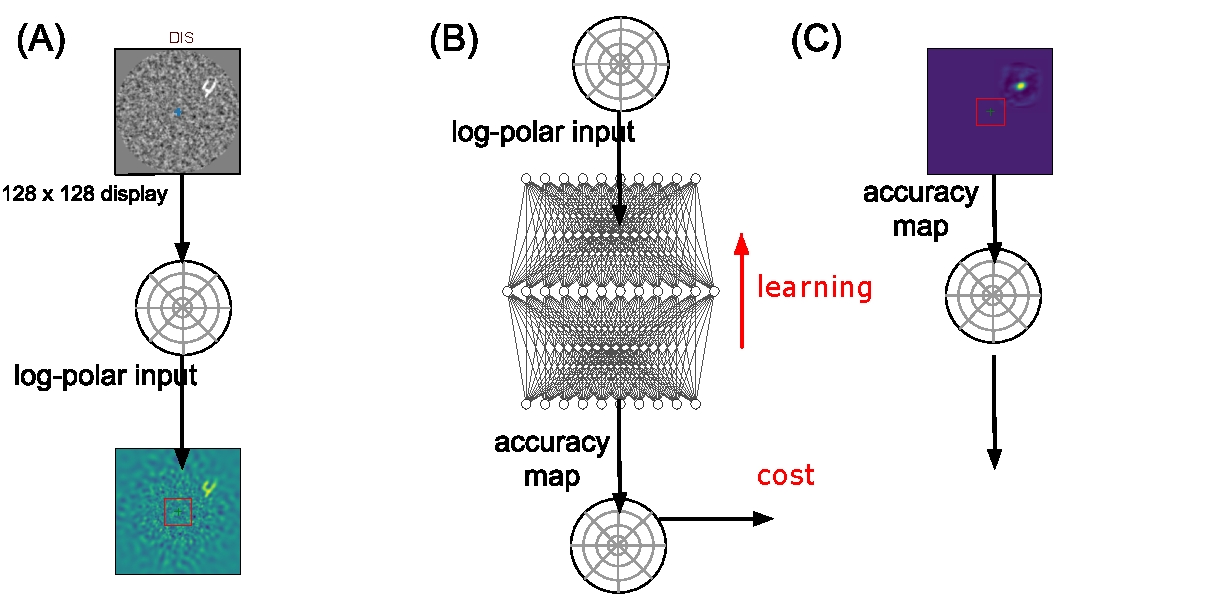
\includegraphics[width=\linewidth]{fig_where.pdf}}
	\caption{Implementing the ``Where'' pathway: \A A visual display is transformed by a feature vector which elements compute the similarity of the full image with a bank of oriented filters placed at positions defined by a log-polar grid. This defines a linear transform of the $128\times128=16384$ input pixels into $2880$ coefficients. It is possible to represent this information in visual space by using the pseudo-inverse of the linear transform (see for instance Figure~\ref{fig:intro}-C).
	\B The ``Where'' network consists of two hidden layer composed with a RELU operator transforming the retinal feature vector. A sigmoid operator ensures that this output vector is a distribution of predicted probabilities in log-polar space.  % {\color{magenta} [[\textbf{laurent:} pourquoi on utilise pas un soft-max - on sait qu'il y a une et une seule cible}
	\C Similarly to~(A), any full accuracy map computed by shifting the know shift-dependent accuracy map of the ``What'' pathway (see figure~\ref{fig:accuracy}) can be transformed into a distribution in log-polar space, similarly to a collicular representation. As the full accuracy map is itself a distribution, This can be implemented by a linear (matrix) transform. In practice, one can use the inverse of this linear transform to project any  collicular representation into the visual space, for instance to predict for the position with maximal accuracy (red cross).
	}
\label{fig:where}
\end{figure}

%
% page 476 de :
%
% https://www.asc.ohio-state.edu/golubitsky.4/reprintweb-0.5/output/papers/6120261.pdf
%
% Estimates ofw0D0.087 and2D0.051 inappropriate units can be obtained from Drasdo’s data on the human retina,andaandbare constants. These values correspond to a magnification factor of 11 .5 mm/degrees of visual angle at the fovea and 5.75 mm/degrees
%An interesting perspective is given with previous modeling of such foveated sensors.
% {\color{magenta} [[\textbf{Rev 1} : I think it would be better to first simply describe the architecture of the pathway (linear filters with retinotopic distribution, linear operation (??) and sigmoid to predict local accuracies) and then go into more detail on why the different parts where designed in a certain way. Also, maybe a figure that shows more architectural details of the "where"-pathway than figure 2 might be helpful.]]}
% TODO : add a figure showing the architecture of the V1 feature vector + where pathway ?
Here, we assume the ``Where'' implements the following action selection: where to look next in order to reduce the uncertainty about the target identity?
The ``Where'' pathway is thus devoted to choosing the next saccade by predicting the location of the target in the (log-polar) visual field.
This implies moving the eye such as to increase the ``What'' categorization accuracy. For a given visual field, each possible future saccade has an expected accuracy, that can be trained from the ``What'' pathway output. To accelerate the training, we use a shortcut that is training the network on a translated accuracy map. The output is thus an accuracy map, that tells for each possible visuomotor displacement the value of the future accuracy.

\paragraph{Primary visual representation: log-polar orientation filters}
In order to reduce the processing cost, and in accordance with observations~\cite{connolly1984representation,sparks1987sensory}, a similar log-polar compression pattern is assumed to be conserved from the retina up to the primary motor layers.
The non-uniform sampling of the visual space is adequately modeled as a log-polar conformal mapping, as it provides a good fit with observations in mammals~\cite{Traver10} which has a long history in computer vision and robotics.
%A first property of this mapping is the separation between the foveal and the peripheral areas as we defined above.  However, this sensor is to our knowledge most often not coupled to an action.
%\if 0\ICANN
% {\color{blue}(but see~\cite{ref_needed)}}\fi.
Both the visual features and the output accuracy map are to be expressed in retinal coordinates.
% {\color{magenta} [[ \textbf{Rev 1} It would be very helpful to have at least a little bit more details on what the log-polar oriented filters are. Right now there is only a reference to [28].]]}
On the visual side, local visual features are extracted as oriented edges as a combination of the retinotopic transform with primary visual cortex filters~\cite{Fischer2007a}, see Figure~\ref{fig:where}-A. The centers of these first and second order orientation filters are radially organized around the center of fixation, with small and tightened receptive fields at the center and more large and scarce receptive fields at the periphery.
% see Figure~\ref{fig:methods}-B.
The size of the filters increases proportionally to the eccentricity.  The filters are organized in $10$ spatial eccentricity scales (respectively placed at around $2$, $3$, $4.5$, $6.5$, $9$, $13$, $18$, $26$, $36.5$ , and $51.3$ pixels from the center) and $24$ different azimuth angles allowing them to cover most of the original $128 \times 128 $ image. At each of these positions, $6$ different edge orientations and $2$ different phases (symmetric and anti-symmetric) are computed. This finally implements a (fixed) bank of linear filters which models the receptive fields of the primary visual cortex.

To ensure the balance of the coefficients across scales, the images are first whitened and then linearly transformed into a retinal input as a feature vector $\boldsymbol{x}$.  The length of this vector is $2880$, such that the retinal filter compresses the original image by about $83\%$, with high spatial frequencies preserved at the center and only low spatial frequencies conserved at the periphery. In practice, the bank of filters is pre-computed and placed into a matrix for a rapid transformation of input batches into feature vectors. This matrix transformation allows also the evaluation of a reconstructed visual image given a retinal activity vector thanks to a pseudo-inverse of the forward transform matrix. In summary, the full-sized images are transformed into a primary visual feature vector which is fed to the ``Where'' pathway.

\paragraph{Visuo-motor representation: ``Collicular'' accuracy maps}

The output of the ``Where'' pathway is defined as an \emph{accuracy map} representing the recognition probability after moving the eye, independently of its identity. Like the primary visual map, this target accuracy map is also organized radially in a log-polar fashion, making the target position estimate more precise at the center and fuzzier at the periphery. This modeling choice is reminiscent of the approximate log-polar organization of the superior colliculus (SC) motor map~\cite{sparks1987sensory}. To ensure that this output is a distribution function, we use a sigmoid operator at the ouput of the ``Where'' network. In ecological conditions, this accuracy map should be trained by sampling, i.e. by ``trial and error'', using the actual recognition accuracy (after the saccade) to grade the action selection. For instance, we could use corrective saccades to compute (a posteriori) the probability of a correct localization. In a computer simulation however, this induces a combinatorial explosion which does render the calculation not amenable.

In practice, as we designed the generative model for the visual display, the position of the target (which is hidden to the agent) is known. Combining this translational shift and the shift-dependent accuracy map of the ``What'' classifier (Figure~\ref{fig:accuracy}-B), the full accuracy map at each pixel can be thus predicted for each visual sample under an ergodic assumption, by shifting the central accuracy map on the true position of the target (see Figure~\ref{fig:where}-C). Such a computational shortcut is allowed by the independence of the categorical performance with position. % {\color{magenta} \textbf{Rev 1 I don't really understand : }}{\color{blue}
This full accuracy map is a probability distribution function defined on the rectangular grid of the visual display. We project this distribution on a log-polar grid to provide the expected accuracy of each hypothetical saccade in a retinotopic space similar to a collicular map. In practice, we used Gaussian kernels defined in the log-polar space as a proxy to quantify the projection from the metric space to the retinotopic space. This generates a filter bank at $10$ spatial eccentricies and $24$ different azimuth angles, i.e. $240$ output filters. To ensure keeping a distribution function, each filter is normalized such that the value at each log-polar position is the average of the values which are integrated in visual space. Applied to the full sized ground truth accuracy map computed in metric space, this gives an accuracy map at different location of a retinotopic motor space. %Such transform is again implemented by a simple matrix multiplication which can be pre-computed to fasten calculations. Practically, this also allows to compute an inverse transform using the pseudo-inverse matrix of the forward transform. In particular, that inverse transform is used to represent the accuracy predicted by any given visual feature vector, but also to compute the position of maximal accuracy in metric space to set up the sensor displacement.

%\subsection{Implementing the ``Where'' pathway}
%=================================================================

\paragraph{Classifier training}
The ``Where'' pathway is a function transforming an input retinal feature vector $\boldsymbol{x}$ into an output log-polar retinotopic vector $\boldsymbol{a}$ representing for each area of the log-polar visual field a prediction of the accuracy probability. Following the active inference framework, the network is trained to predict the likelihood $\boldsymbol{a}_i$ at position $i$ knowing the retinal input $\boldsymbol{x}$ by comparing it to the known ground truth distribution computed over the motor map.
% {\color{magenta} \textbf{Rev 1} According to line 409 the loss function of the classifier is a KL-divergence. However, neither the output of the accuracy map nor the retinotopic vector a are distributions. As far as I understood the, they encode a probabilities for each location. So I don't really see how a KL-divergence could be applicable here.}
The loss function that comes naturally is the Binary Cross-Entropy. At each individual position $i$, this loss corresponds to the negative term of Kullback-Leibler divergence for a binomial random variable $\boldsymbol{a}_i$ given by the predicted map and the ground truth (see Figure~\ref{fig:where}-B).  The total loss is the average over all positions $i$. This scalar measures the distance between both distributions, it is always positive and null if and only if they are equal.

The parametric neural network consists of a primary visual input layer, followed by two fully connected hidden layers of size 1000  with rectified linear activation, and a final output layer with a sigmoid nonlinearity to ensure that the output is compatible with a likelihood function (see Figure~\ref{fig:where}-B). An improvement in convergence speed was obtained by using batch normalization. The network is trained on $60$ epochs of $60000$ samples, with a learning rate equal to $10^{-4}$ and the Adam optimizer~\cite{kingma2014adam} with standard momentum parameters. The full training takes about $1$ hour on a laptop. The code is written in Python (version 3.7.6) with pyTorch library~\cite{NEURIPS2019_9015} (version 1.1.0). The full scripts for reproducing the figures and explore the results to the full range of parameters is available at \url{https://github.com/laurentperrinet/WhereIsMyMNIST}. % TODO: change to https://github.com/SpikeAI/DauceAlbigesPerrinet2020 when public

\paragraph{Quantitative role of parameters}
%: effect of contrast


%: scanning of other parameters
In addition, we controlled that the training results are robust to changes in an individual experimental or network parameters from the default parameters (see Figure~\ref{fig:params}). From the scan of each of these parameters, the following observations were remarkable. First we verified that accuracy decreased when \texttt{noise} increased and while the bandwidth of the noise imported weakly, the spatial frequency of the noise was an important factor. In particular, final accuracy was worst for a clutter spatial frequency of $\approx 0.07$, that is when the characteristic textures elements were close to the characteristic size of the objects. Second, we saw that the dimension of the ``Where'' network was optimal for a dimensionality similar to that of the input but that this mattered weakly. The dimensionality of the log-polar map is more important. The analysis proved that an optimal accuracy was achieved when using a number of $24$ azimuthal directions. Indeed, a finer log-polar grid requires more epochs to converge and may result in an over-fitting phenomenon hindering the final accuracy. Such fine tuning of parameters may prove to be important in practical applications and to optimize the compromise between accuracy and compression.
%=================================================================
%------------------------------%
%: see Figure~\ref{fig:params}
\begin{figure}[t!]%%[p!]
	\centering{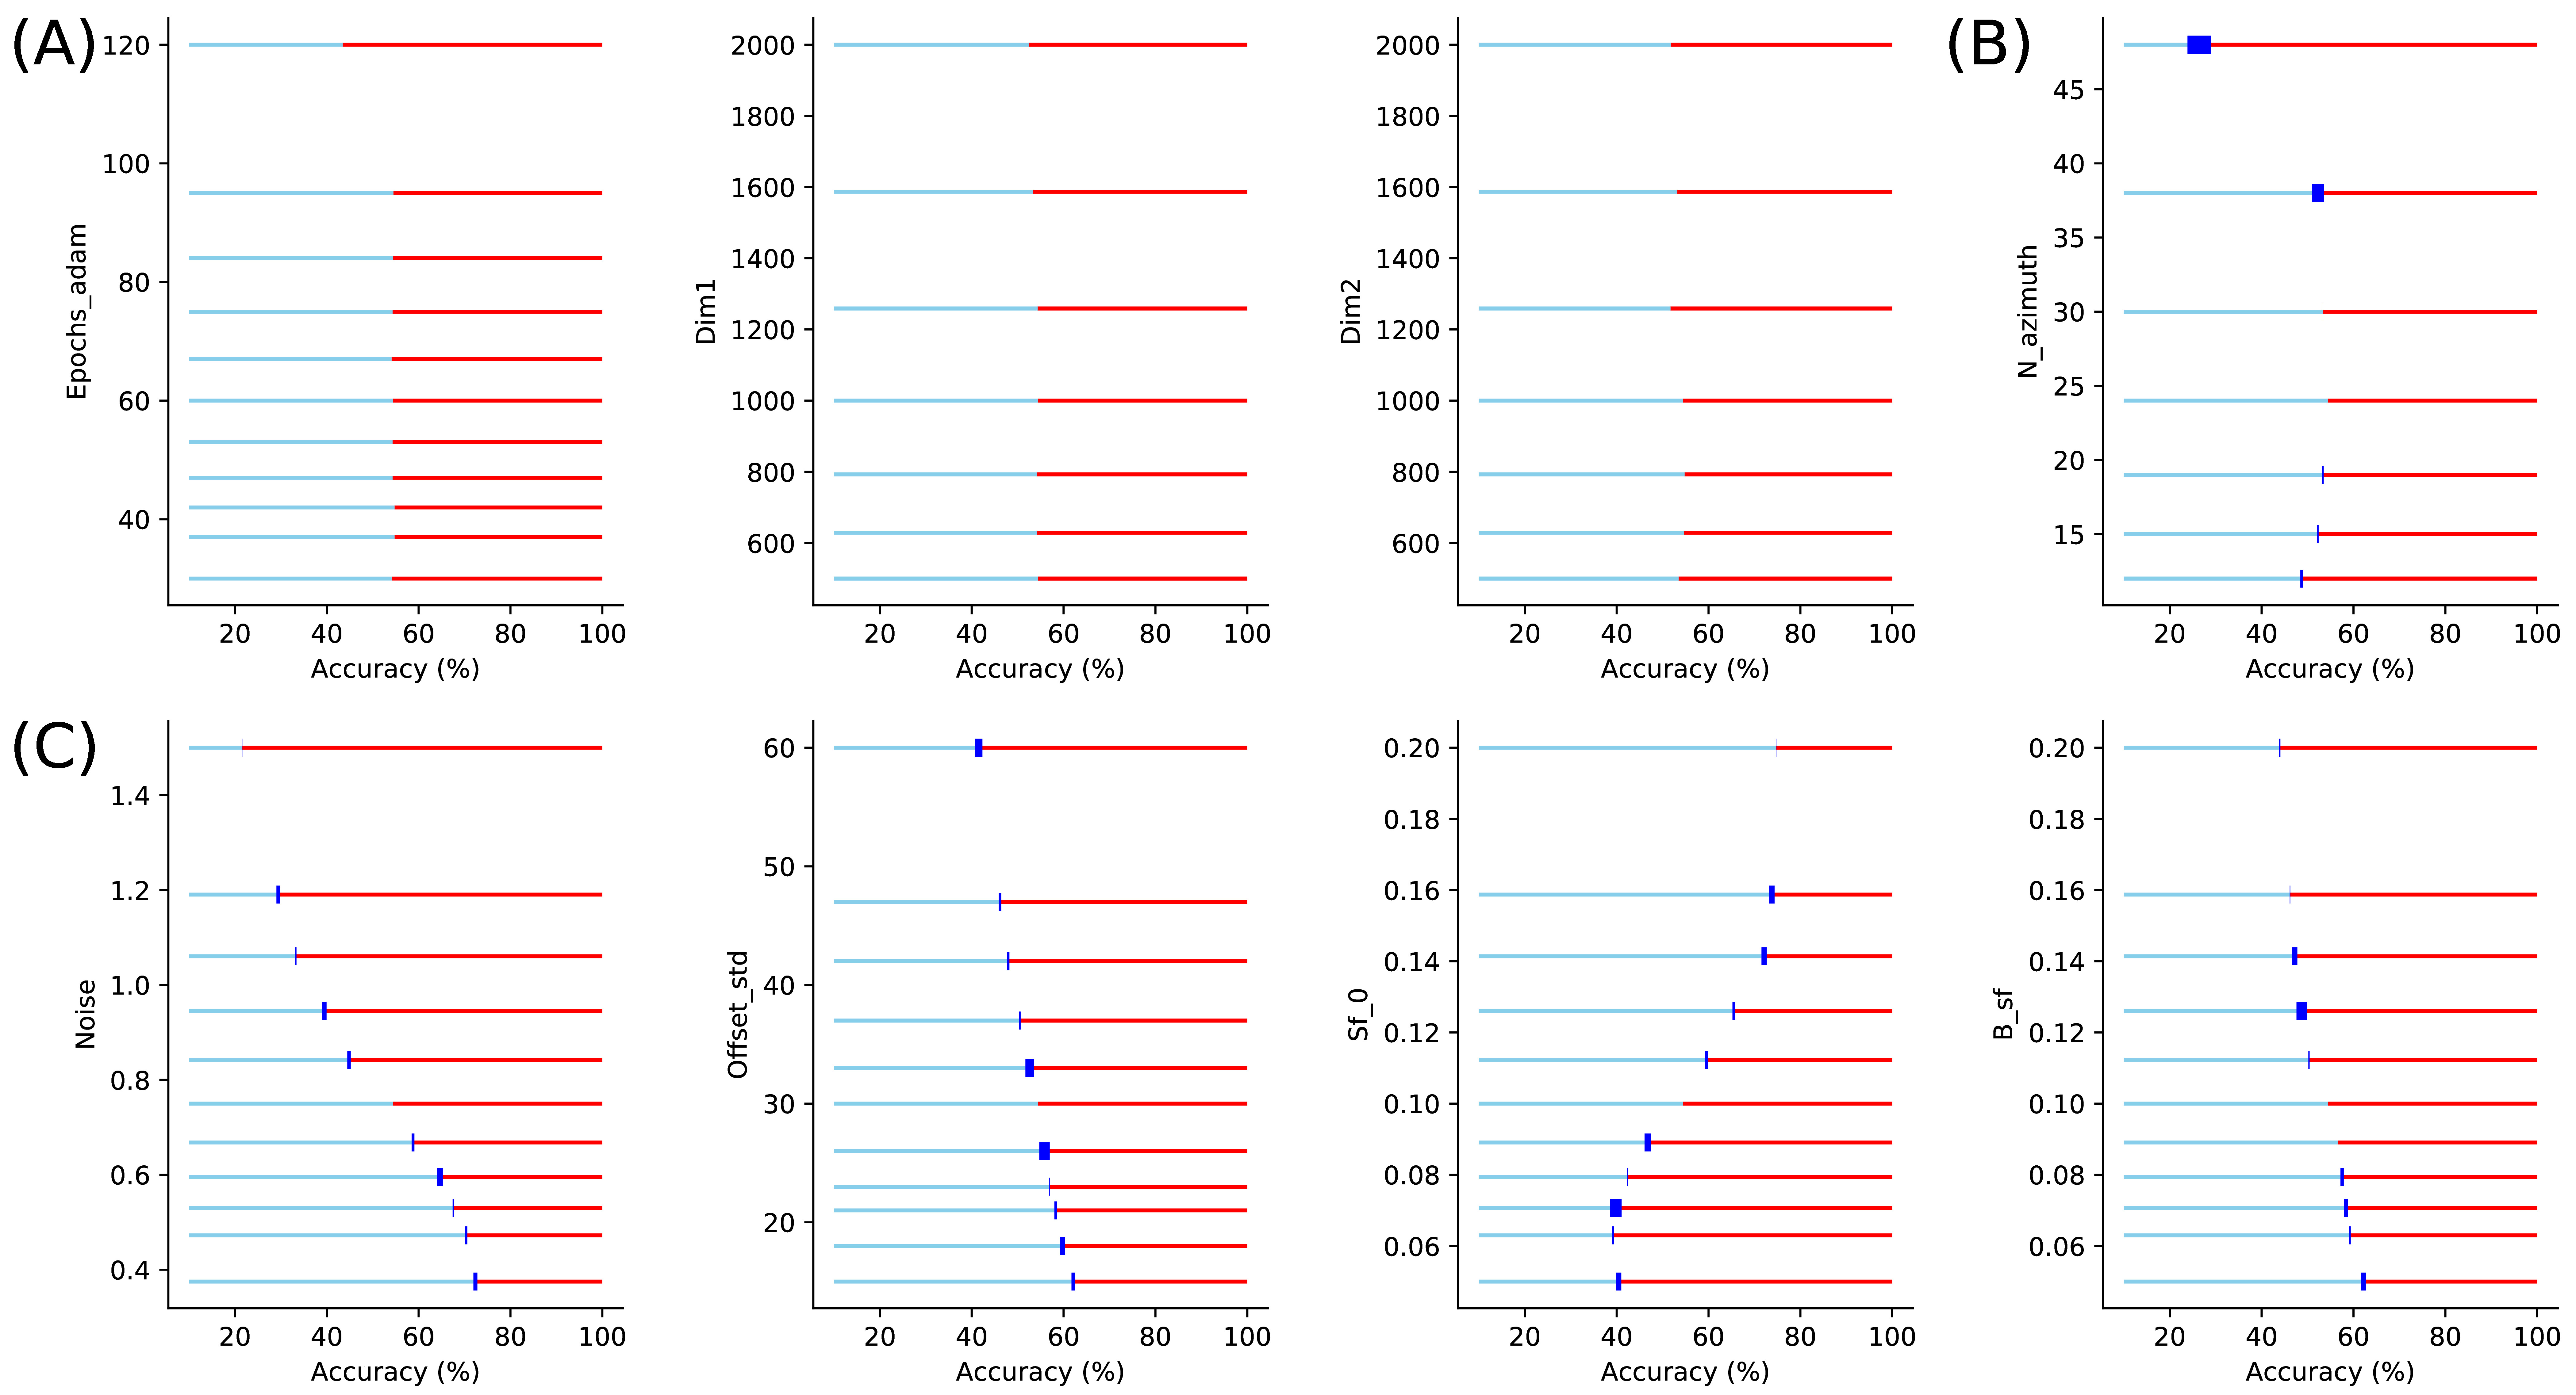
\includegraphics[width=\linewidth]{fig_params}}
	\caption{
		{\bf Quantitative role of parameters}:
		% {\color{magenta} \textbf{Rev 1}
		% 	I have problems understanding Figure 7:
		% 	(1) Accuracy should be the dependent variable, correct? Then I would expect it to be on the y axis, not the x axis
		% 	(2) What are the horizontal lines? What do the different colors mean? Why is there sometimes a little marker at the border between the two colors?
		% 	(3) does the figure include dependency on the hyperparameters of the log-polar filters, i.e., number of eccentricities, number of orientations, ...? If not: I think this would be very important to check.
		% }
		% {\color{red} \textbf{Rev2}
		% In Figure 7, what do the blue and red colors mean? There could be several ways to interpret these plots. Please improve the plots and the caption for clarity. Also, the cases B and C are mixed up.}
		We tested all parameters of the presented model, from that controlling the architecture of image generation, to the parameters of the neural network implementing the ``Where'' pathway (including meta-parameters of the learning paradigm). We show here the results which show the most significative impact on average accuracy.
		The accuracy is given by a blue line, the red line giving the rate of errors. The black dashed line gives the chance level ($10\%$), while the blue box gives the $99\%$ confidence interval as estimated over $8$ repetitions of the learning. %
		%We show here variations of the average accuracy as a function of free parameters of the model. %
		\A First, we tested some properties of the input, respectively from left to right: noise level (\texttt{Noise}), standard deviation  of the distance of the target with respect to the fixation (\texttt{Offset\_std}), mean spatial frequency of clutter \texttt{Sf\_0} and bandwidth \texttt{B\_sf} of the clutter noise. This shows that average accuracy evolves with noise (see also Figure~\ref{fig:results} for an evolution as a function of eccentricity), but also to the characteristics of the noise clutter. In particular, there is a drop in accuracy whenever noise is of similar wavelength as digits, but which becomes less pronounced as the bandwidth increases. %
		\B Finally, we scanned parameters of the Deep Learning neural network. We observed that accuracy quickly converged after approximately $25$ epochs (\texttt{Epochs\_adam}). We then tested different values for the dimension of respectively the first (\texttt{Dim1}) and second (\texttt{Dim2}) hidden layers, showing weak changes in accuracy. %
		\C
		The accuracy also changes with the architecture of the foveated input as shown here by changing the number \texttt{N\_azimuth} of azimuth directions which are sampled in visual space. This shows a compromise between a rough azimuth representation and a large precision, which necessitates a longer training phase, such that the optimal number is around $24$ azimuth directions. %
		\label{fig:params}}%
\end{figure}%
%%------------------------------%

% TODO : make a (minimal) psychophysics experiment= show an image as in figure 1, then in (ANS), make a 2AFC task by showing the true versus a random one -> web experiment using pavlovia?


\subsection{Concurrent action selection}
\label{sec:IG}

Finally, when both pathways are assumed to work in parallel, each one may be used concurrently to choose the most appropriate action. Two concurrent accuracies are indeed  predicted through separate processing pathways, namely the central pixels recognition accuracy through the ``What'' pathway, and the log-polar accuracy map through the ``Where'' pathway. The central accuracy may thus be compared with the maximal accuracy as predicted by the ``Where'' pathway.

From the information theory standpoint, each saccade comes with fresh visual information about the visual scene that can be quantified by a conditional \emph{information gain}, namely:
\begin{align}
\text{IG}_\text{max} &= \max_{x'} \log p(y|x,x') - \log p(y|x)\nonumber
\end{align}
with the left term representing the future accuracy (after the saccade is realized) and the right term representing the current accuracy as it is obtained from the ``What'' pathway.
Estimating the joint conditional dependence in the first term being once again out of reach for computational reasons, the following approximative estimate is used instead {\color{green} à justifier un peu mieux}:
\begin{align}
\tilde{\text{IG}}_\text{max}&\simeq \text{IG}_\text{max}\nonumber\\
&=\max_{x'} \log p(y|x') - \log p(y|x)\label{eq:IG}
\end{align}
that is a simple difference between the log accuracy after the saccade minus the log accuracy before the saccade.
To provide a reliable estimate, the information gain may be averaged over many saccades and many target eccentricities (so that the information gain may be close to zero when the target eccentricity is close to zero).
For the saccade is subject to predictions errors and execution noise, the saccade landing position may be different from the initial prediction. The final accuracy, as instantiated in the accuracy map, contains this intrinsic imprecision, and is thus necessary lower than the optimal one. The consequence is that in some cases, the approximate information gain may become negative, when the future accuracy is actually lower than the current one. This is for instance the case when the target is exactly positioned at the center of the fovea.
